\documentclass[11pt]{article}

\usepackage{bbm}
\usepackage{geometry}
\usepackage{graphicx}
\usepackage{amsmath}
\usepackage{float}
\usepackage{listings}
\usepackage{indentfirst}
\usepackage{braket}
\usepackage{authblk}
\usepackage{hyperref}
\setlength{\parindent}{2em}
\geometry{left=2.5cm,right=2.5cm,top=2.0cm,bottom=2.0cm}
% About the author
\renewcommand*{\Authand}{, }
\renewcommand\Affilfont{\itshape\small}
\lstset{language=C}

\date{}

\title{Memory Usage and Time Consumption in Diagonalizing Matrix}
\author[1]{Zeyuan Ye}
\setcounter{Maxaffil}{0}

\begin{document}
  \maketitle

\begin{abstract}
This note aims at finding the functional relation of memory usage and time costing with
matrices’ sizes in diagonalization. The first method represents the largest matrix one can diagonalize on a
computer. Yet one might need to do this testing again once the computer varied. On the other
hand, the second method can give a universal functional relation of memory usage and matrix size,
although with some inaccuracy. Time consumption of diagonalizing can vary much depends on
the quality of the matrix. Brief results of this note are included in the Summary section.
\end{abstract}

\section{Testing information}
Diagonalizing is done by MKL functions: LAPACKE\_dgehrd and LAPACKE\_dhseqr.
LAPACKE\_dgehrd is used for converting general matrix into a Hessenberg matrix and
LAPACKE\_dhseqr can do the the Schur factorization , in which one can get the
eigenvalues from the upper matrix easily. Details are covered in
\cite{lapack, lapack2}. I packed these two functions up as function \textit{findEigenValue} in
\textit{TEG\_Faddeev/src/tool/matOperator.cpp}.
MKL's version is 2019.1.144.

As for testing codes and how to use them, please read \textit{TEG\_Faddeev/test/testTemp/readMe.org}

\section{Memory Usage: Method 1}
This method is straightforward but powerful: try it manually. If there are memory
errors, GNU will print out the error message immediately. To ensure the matrix being
diagonalized correctly, one also need to print out the eigenvalues and check them.

The drawback of this method is apparent as well: test needs to be done every time
when computer changes. Considering the large size of matrix, this would be a
time-consuming task. 

In addition, large matrix size need long type as the index variables.
\section{Memory Usage: Method 2}
This method aims at finding a functional relation. Because there seems no
simple function in C++ can catch the memory and swap information reliably, I used command
\textit{free -m} in the shell script, and then run it with C++ codes spontaneously.
Data analysis was done by shell script and python.
These procedures were packed in command \textit{testServerMem} in \textit{TEG\_Faddeev/src/test/testTemp/makefile}. Figure \ref{mem} shows the results. 

\begin{figure}[H]
\centering
\begin{minipage}[c]{0.5\textwidth}
\centering
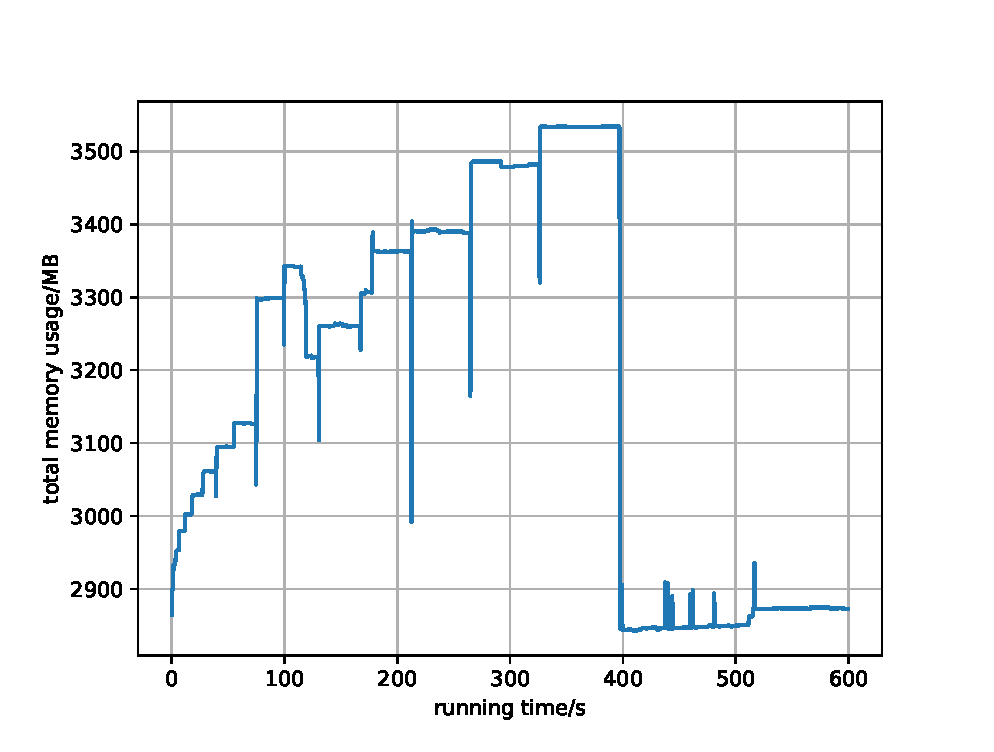
\includegraphics[height=6.5cm]{memRaw.eps}
\put(-70,120){(a)}
\end{minipage}%
\begin{minipage}[c]{0.5\textwidth}
\centering
\includegraphics[height=6.5cm]{memFit.eps}
\put(-70,120){(b)}
\end{minipage}
\caption{(a) Raw data catched by \textit{free -m}. Sampling frequency is 5Hz with total 3000 samples be catptured. Y axis
  is the sum of memory and swap usage. Notice a large potion of it is used
  by the system. (b) Fitting function. There is a jump at size = $4500^2$.}
\label{mem}
\end{figure}

Roughly speaking, memory usage depends on the size of matrix linearly as one
might expect. However, there is a jump around $\text{size} = 4500^2$. If this jumping doesn't occur frequently, the linear function is
good enough to estimate the memory usage. To verify this result, I tried a
matrix with size $15000 \times 15000$. The theoritical prediction is about
$4000$ MB, which is very close to the experiment result, around $3900$ MB, .

\section{Time Consumption}

This is much easier, just record time and analyze them in Python. Figure \ref{time}
is the result.

\begin{figure}[H]
\centering
\begin{minipage}[c]{0.5\textwidth}
\centering
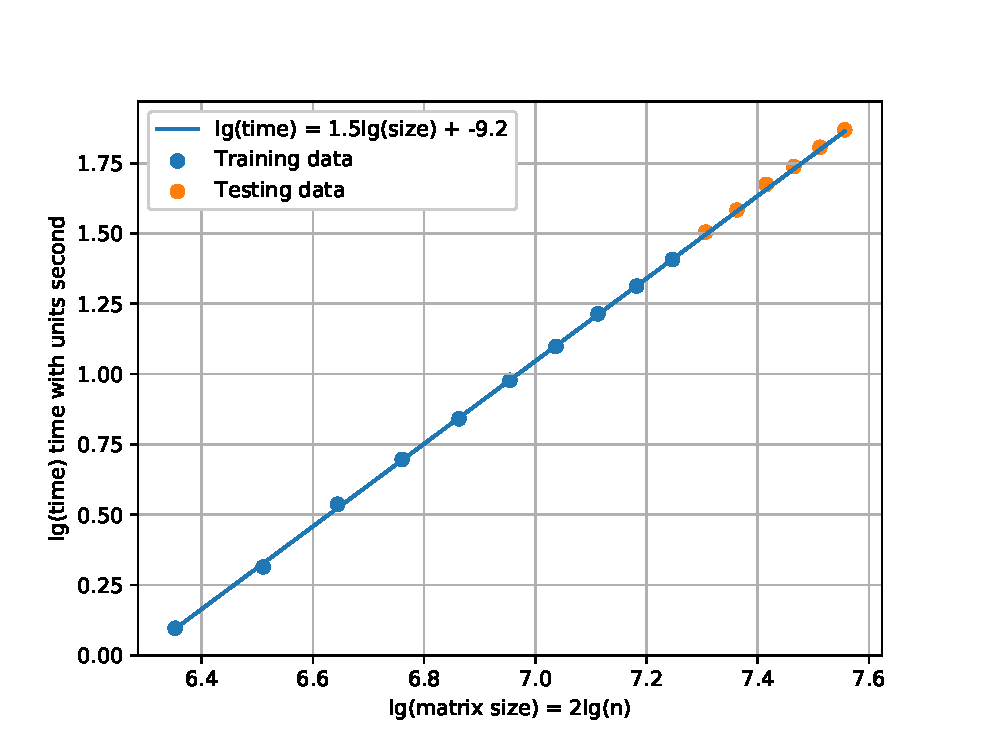
\includegraphics[height=6.5cm]{time0.eps}
\put(-70,120){(a)}
\end{minipage}%
\begin{minipage}[c]{0.5\textwidth}
\centering
\includegraphics[height=6.5cm]{time1.eps}
\put(-70,120){(b)}
\end{minipage}
\caption{(a)(b) Fitting functions with matrices with elements all 0s and all 1s
  separately.}
\label{time}
\end{figure}

Time consumption can vary largely depends on the quality of the matrix. For
diagonalized matrix (includes matrix with all 0), time depends on $size^{1.5}$. On
the other hand, matrix with all elements 1 need time consumption proportional to $size^2$. 

\section{Summary}

The following data is about the capacity of the server, with only eigenvalues
are computed.
\begin{itemize}
\item{Memory usage function (unit = bytes): $mem = 16.8 n^2 + b_0$ to $ 19.8 n^2 + b_0$}
\item{Time consumption (unit = seconds) function for matrix with elements all 0s: $10^{-12.9}
    n^{3.7}$.}
\item{Time consumption function for matrix with elements all 1s: $10^{-11.2} n^{3.7}$}
\end{itemize}
where matrix size is $n^2$, $b_0$ is the memory usage without any calculation.
You can read it thought command \textit{free -m}. It's about 600 MB in the
server.

In all, one can conclude the following (all elements in matrix are 1s), 
\begin{itemize}
\item{Maximum size of matrix: $80600^2$}
\item{Size of matrix that can be diagonalized in 1 hour: $9731^2$}
\item{Size of matrix that can be diagonalized in 1 day: $22973^2$}
\end{itemize}
The maximum size of matrix has been verified though Method 1 directly.

\begin{thebibliography}{100}
  \bibitem{lapack}
    \url{https://software.intel.com/en-us/mkl-developer-reference-c-nonsymmetric-eigenvalue-problems-lapack-computational-routines}
    \bibitem{lapack2}
    \url{https://software.intel.com/en-us/mkl-developer-reference-c-hseqr}
\end{thebibliography}

\end{document}

